% lualatex presentation

\documentclass[svgnames]{beamer}
\usepackage[utf8]{inputenc}
\usepackage{fontspec}
\usepackage{arev}
\usepackage{beramono}
\usepackage{fontawesome}
\usepackage{pifont}
\usepackage{rotating}
\usepackage{listings}
\usepackage{ulem}
\usepackage{hyperref}

\usetheme{default}
\setbeamertemplate{navigation symbols}
{%
%  \hspace{3em}
%  \vbox{%
%  \hbox{\insertslidenavigationsymbol}
%  \hbox{\insertframenavigationsymbol}
%  \hbox{\insertbackfindforwardnavigationsymbol}
%  \vspace{2em}}
}

\setbeamercolor{alerted text}{fg=red!70!black}
\setbeamercolor{structure}{fg=Navy}


\hypersetup{%
  pdftitle={Introduction to NumPy arrays}
  ,pdfauthor={Gert-Ludwig Ingold <gert.ingold@physik.uni-augsburg.de>}
  ,pdfsubject={Tutorial at EuroSciPy 2016, Erlangen 23.8.2016}
  ,pdfkeywords={Python, NumPy, tutorial, EuroSciPy}
}

\lstset{%
  language=Python
  ,basicstyle={\ttfamily}
  ,escapechar=/
}

\newfontfamily\DejaSans{DejaVu Sans}
\definecolor{positive}{rgb}{0, 0.5, 0}
\definecolor{negative}{rgb}{0.7, 0, 0}
\newcommand\smiley{\textcolor{positive}{\DejaSans ☺}}
\newcommand\frownie{\textcolor{negative}{\DejaSans ☹}}

\newcommand{\soutthick}[1]{%
  \renewcommand{\ULthickness}{1.5pt}%
  \sout{#1}%
  \renewcommand{\ULthickness}{.4pt}% Resetting to ulem default
}

\graphicspath{{./images/}}

\begin{document}

\begin{frame}
 \begin{center}
  \structure{\Large\textbf{Introduction to NumPy arrays}}\\[0.3truecm]
  \structure{\large Gert-Ludwig Ingold}

  \vspace{2truecm}
  \faicon{github}\ \ttfamily{\footnotesize https://github.com/gertingold/euroscipy16-numpy-tutorial.git}
 \end{center}
\end{frame}

\begin{frame}[t]{Python comes with batteries included}
 \ding{220} extensive Python standard library

 \vspace{0.3truecm}
 \structure{What about batteries for scientists (and others as well)?}

 \vspace{0.2truecm}
 \ding{220} scientific Python ecosystem

 \begin{center}
  \only<1>{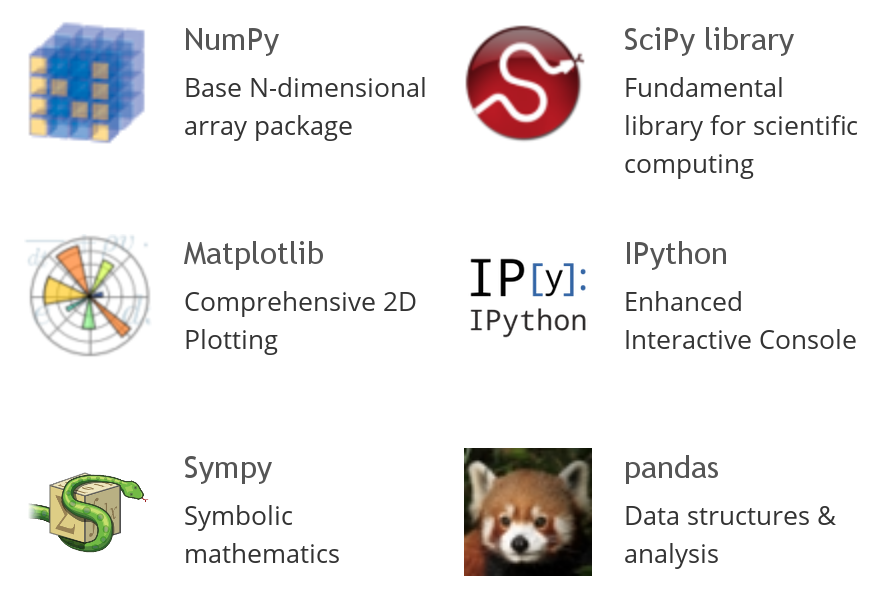
\includegraphics[width=0.7\textwidth]{SciPyEco}}%
  \only<2>{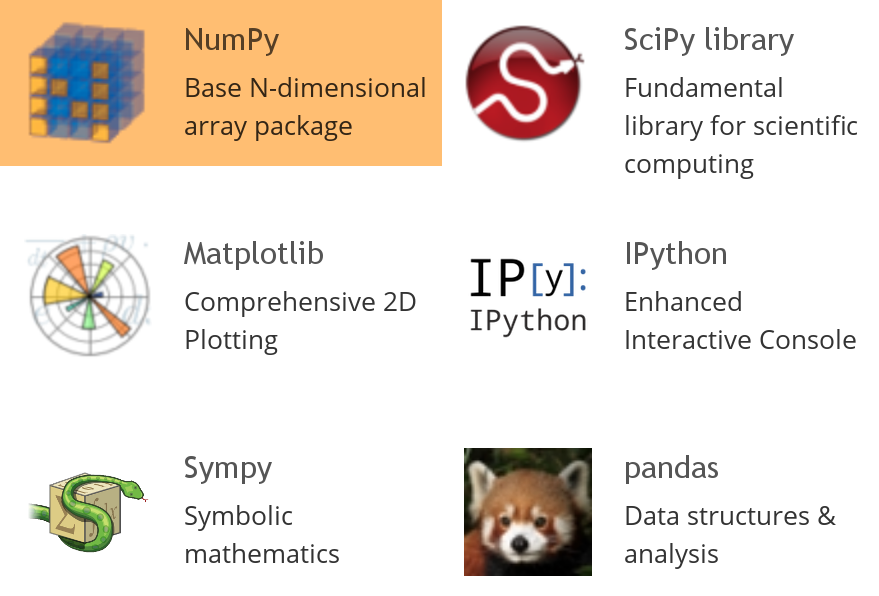
\includegraphics[width=0.7\textwidth]{SciPyEco_NumPy}}\quad%
  \raisebox{0.2truecm}{%
   \begin{sideways}
    \tiny from: \url{www.scipy.org}
   \end{sideways}}
 \end{center}

 + SciKits and many other packages
\end{frame}

\begin{frame}
 \vspace*{-0.5truecm}
 \begin{columns}
  \begin{column}[t]{0.5\textwidth}
   \begin{center}
    \structure{www.scipy-lectures.org}

    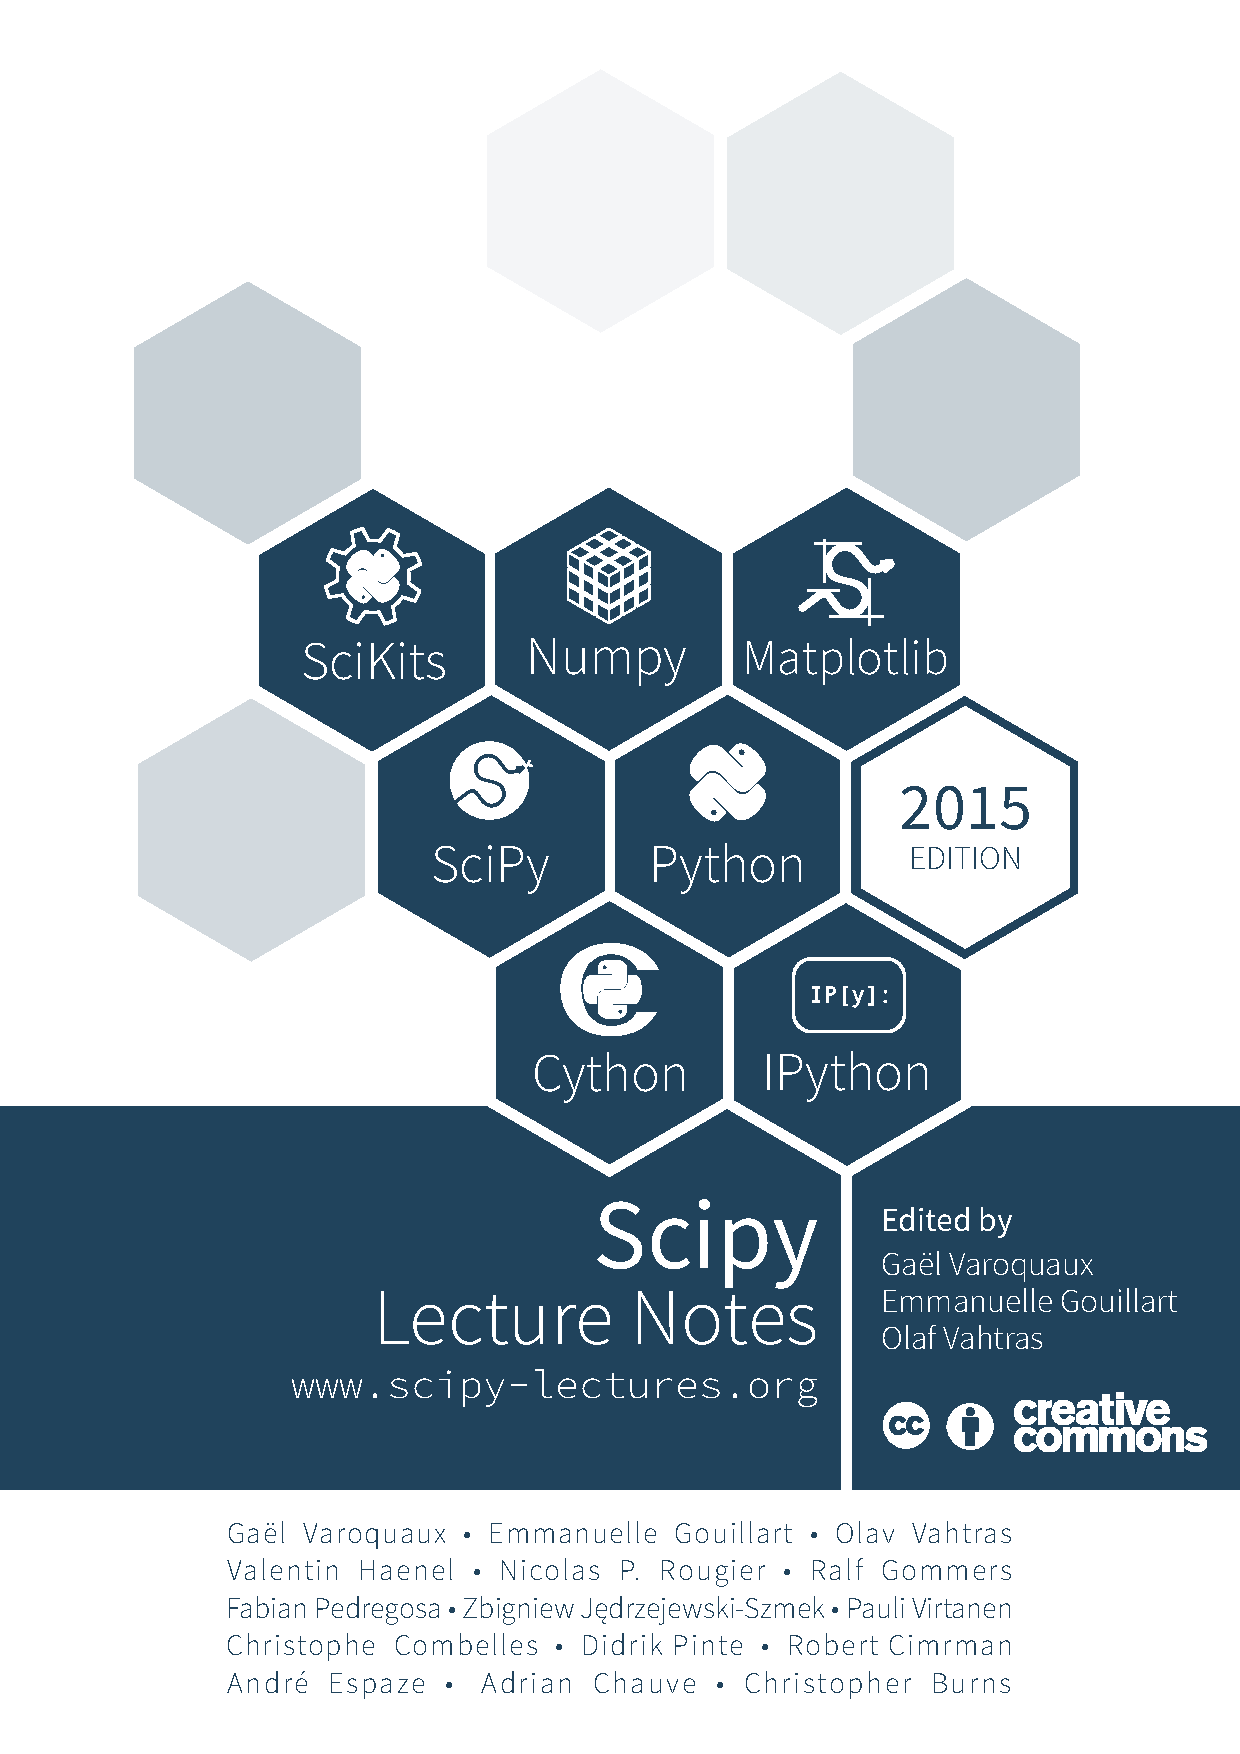
\includegraphics[width=\textwidth]{ScipyLectCover}
   \end{center}
  \end{column}%
  \begin{column}[t]{0.5\textwidth}
   \begin{center}
    \structure{docs.scipy.org/doc/numpy/}

    \vspace{0.3truecm}
    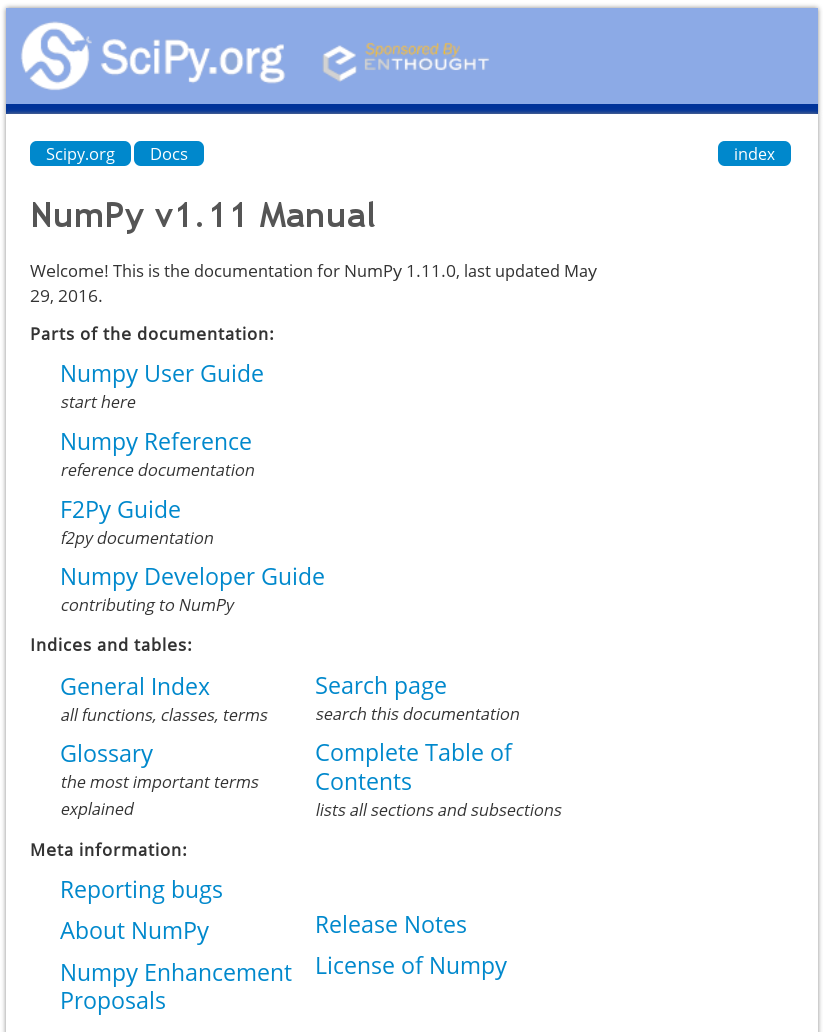
\includegraphics[width=\textwidth]{NumpyManual}
   \end{center}
  \end{column}
 \end{columns}
\end{frame}

\begin{frame}{A wish list}
 \begin{itemize}
  \item we want to work with vectors and matrices
 \end{itemize}

 \begin{columns}
  \begin{column}{0.55\textwidth}
   \begin{displaymath}
    \begin{pmatrix}
     a_{11} & a_{12} & \cdots & a_{1n}\\
     a_{21} & a_{22} & \cdots & a_{2n}\\
     \vdots & \vdots & \ddots & \vdots\\
     a_{n1} & a_{n2} & \cdots & a_{nn}\\
    \end{pmatrix}
   \end{displaymath}
  \end{column}%
  \begin{column}{0.45\textwidth}
   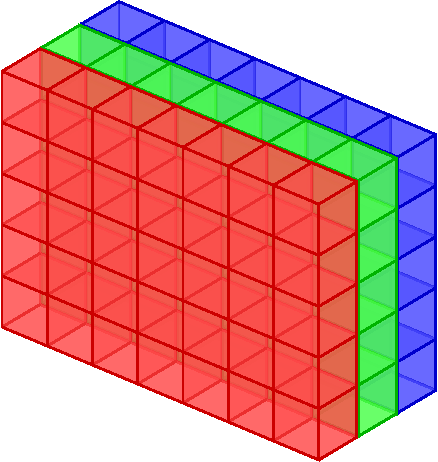
\includegraphics[width=0.7\textwidth]{rgbarray}

   colour image as $N\times M\times3$-array
  \end{column}
 \end{columns}

 \begin{itemize}
  \item we want our code to run fast
  \item we want support for linear algebra
  \item \dots 
 \end{itemize}
\end{frame}

\begin{frame}{List indexing}
 \begin{center}
  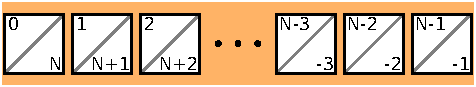
\includegraphics[width=0.96\textwidth]{listindexing2}
 \end{center}
 \begin{itemize}
  \item indexing starts at 0
  \item negative indices count from the end of the list to the beginning
 \end{itemize}
\end{frame}

\begin{frame}{List slicing}

 basic syntax: \texttt{[start:stop:stride]}

 \vspace{0.2truecm}
 \begin{center}
  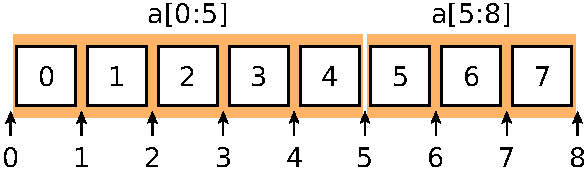
\includegraphics[width=\textwidth]{listindexing1}
 \end{center}
 \begin{itemize}
  \item slice contains the elements \texttt{start} to \texttt{stop-1}
  \item slice contains \texttt{stop-start} elements
  \item default values:
  \begin{itemize}
      \item \makebox[1.5truecm]{\texttt{start}\hfill} 0 (first element)
      \item \makebox[1.5truecm]{\texttt{stop}\hfill} N-1 (last element)
      \item \makebox[1.5truecm]{\texttt{stride}\hfill} 1
  \end{itemize}
 \end{itemize}
\end{frame}

\begin{frame}
 \begin{center}
  \structure{\large\bfseries Let's do some slicing}

  \vspace{0.5truecm}
  
\includegraphics[width=3truecm]{yourturn}
 \end{center}
\end{frame}

\begin{frame}[fragile, t]{Matrices and lists of lists}
 
 \vspace{0.3truecm}
 Can we use lists of lists to work with matrices?

 \begin{columns}
  \begin{column}{0.4\textwidth}
   \begin{displaymath}
    \begin{pmatrix}
     0 & 1 & 2\\
     3 & 4 & 5\\
     6 & 7 & 8
    \end{pmatrix}
   \end{displaymath}
  \end{column}%
  \begin{column}{0.6\textwidth}
   \begin{center}
    \begin{lstlisting}%[language=python]
matrix = [[0, 1, 2],
          [3, 4, 5],
          [6, 7, 8]]
    \end{lstlisting}

    \vspace{\baselineskip}
   \end{center}
  \end{column}
 \end{columns}
 \begin{itemize}
  \item How can we extract a row? \uncover<3>{\smiley}
  \item How can we extract a column? \uncover<3>{\frownie}
 \end{itemize}

 \vspace{0.3truecm}
 \begin{center}
  \only<2>{\structure{\large\bfseries Let's do some experiments}

  \vspace{0.5truecm}
  
\includegraphics[width=3truecm]{yourturn}}%
  \only<3>{\alert{Lists of lists do not work like matrices}}
 \end{center}
\end{frame}

\begin{frame}{Problems with lists as matrices}
 \begin{itemize}
  \item different axes are not treated on equal footing
  \item lists can contain arbitrary objects\\
        matrices have a homogeneous structure
  \item list elements can be scattered in memory
 \end{itemize}

 \vspace{0.3truecm}
 Applied to matrices \dots
 \begin{itemize}
  \item[] \dots lists are conceptually inappropriate
  \item[] \dots lists have less performance than possible
 \end{itemize}
\end{frame}

\begin{frame}{We need a new object}

 \begin{center}
  \structure{\Huge\bfseries ndarray}

  \vspace{0.5truecm}
  multidimensional, homogeneous array of fixed-size items
 \end{center}
\end{frame}

\begin{frame}[fragile, t]{Getting started}

 \vspace{1.5truecm}
 Import the NumPy package:

 \vspace{0.4truecm}
 \begin{center}
  \begin{minipage}{0.75\textwidth}
   \only<1>{\texttt{from numpy import *}}%
   \only<2->{\soutthick{\texttt{from numpy import *}}}

   \only<2>{\texttt{from numpy import array, sin, cos}}%
   \only<3->{\soutthick{\texttt{from numpy import array, sin, cos}}}

   \only<3>{\texttt{import numpy}}%
   \only<4->{\soutthick{\texttt{import numpy}}}

   \only<4>{\texttt{import numpy as np}\quad\rotatebox[origin=c]{180}{\alert{\ding{220}}}

            \vspace{0.5truecm}
            \begin{center}
             
\includegraphics[width=3truecm]{yourturn}
            \end{center}}
  \end{minipage}
 \end{center}
\end{frame}

\begin{frame}{Data types}
Some important data types:

\vspace{0.3truecm}
\begin{tabular}{ll}
integer & \texttt{int8}, \texttt{int16}, \texttt{int32}, \texttt{int64}, \texttt{uint8}, \dots\\[0.2truecm]
float   & \texttt{float16}, \texttt{float32}, \texttt{float64}, \dots \\[0.2truecm]
complex & \texttt{complex64}, \texttt{complex128}, \dots\\[0.2truecm]
boolean & \texttt{bool8}\\[0.2truecm]
Unicode string  & \\
\end{tabular}

\vspace{0.3truecm}
Default: Python float

\vspace{0.3truecm}
\begin{center}
 \alert{Beware of overflows!}
\end{center}

\begin{center}
 
\includegraphics[width=3truecm]{yourturn}
\end{center}
\end{frame}

\begin{frame}{Strides}
 \begin{columns}
  \begin{column}{0.33\textwidth}
   \begin{displaymath}
    \begin{pmatrix}
     0 & 1 & 2 & 3 & 4 & 5
    \end{pmatrix}
   \end{displaymath}
  \end{column}%
  \begin{column}{0.67\textwidth}
   (8,)

   \vspace{0.2truecm}
   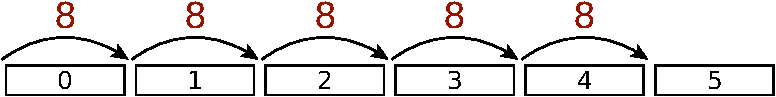
\includegraphics[width=\textwidth]{strides_0}
  \end{column}
 \end{columns}

 \vspace{0.8truecm}
 \begin{columns}
  \begin{column}{0.33\textwidth}
   \begin{displaymath}
    \begin{pmatrix}
     0 & 1 & 2\\
     3 & 4 & 5
    \end{pmatrix}
   \end{displaymath}
  \end{column}%
  \begin{column}{0.67\textwidth}
   (24, 8)

   \vspace{0.2truecm}
   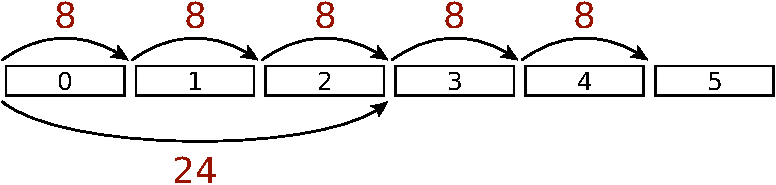
\includegraphics[width=\textwidth]{strides_3}
  \end{column}
 \end{columns}

 \vspace{0.8truecm}
 \begin{columns}
  \begin{column}{0.33\textwidth}
   \begin{displaymath}
    \begin{pmatrix}
     0 & 1 \\
     2 & 3 \\
     4 & 5
    \end{pmatrix}
   \end{displaymath}
  \end{column}%
  \begin{column}{0.67\textwidth}
   (16, 8)

   \vspace{0.2truecm}
   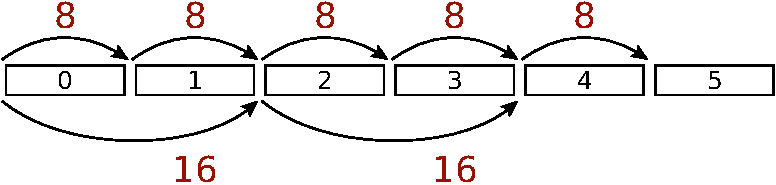
\includegraphics[width=\textwidth]{strides_2}
  \end{column}
 \end{columns}
\end{frame}

\begin{frame}{Views}
 For the sake of efficiency, NumPy uses views if possible.

 \begin{itemize}
  \item Changing one or more matrix elements will change it in all views.
  \item Example: transposition of a matrix \texttt{a.T}\\
        No need to copy the matrix and to create a new one
 \end{itemize}

 \begin{center}
  
\includegraphics[width=3truecm]{yourturn}
 \end{center}
\end{frame}

\begin{frame}{Some array creation routines}

 \begin{itemize}
  \item numerical ranges:
        \texttt{arange}, \texttt{linspace}, \texttt{logspace}
  \item homogeneous data:
        \texttt{zeros}, \texttt{ones}
  \item diagonal elements:
        \texttt{diag}, \texttt{eye}
  \item random numbers:
        \texttt{rand}, \texttt{randint}
 \end{itemize}

 \begin{center}
  
\includegraphics[width=3truecm]{yourturn}
 \end{center}
\end{frame}

\begin{frame}{Indexing and slicing in one dimension}
 \structure{1d arrays}: indexing and slicing as for lists

 \begin{itemize}
  \item first element has index 0
  \item negative indices count from the end
  \item slices: \texttt{[start:stop:step]}\\
        \strut\hphantom{slices:\ }  without the element indexed by \texttt{stop}
  \item if values are omitted:
        \begin{itemize}
         \item \texttt{start}: starting from first element
         \item \texttt{stop}: until (and including) the last element
         \item \texttt{step}: all elements between \texttt{start} and \texttt{stop}-1
        \end{itemize}
 \end{itemize}

 \begin{center}
  
\includegraphics[width=3truecm]{yourturn}
 \end{center}
\end{frame}

\begin{frame}{Indexing and slicing in higher dimensions}
 \begin{itemize}
  \item usual slicing syntax
  \item difference to lists:\\
        slices for the various axes separated by comma
 \end{itemize}

 \begin{center}
  \only<1>{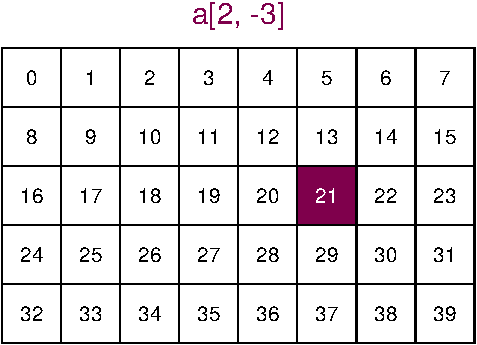
\includegraphics[width=0.8\textwidth]{arraygraphics_0}}%
  \only<2>{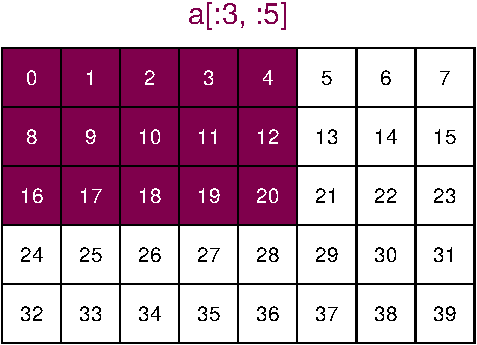
\includegraphics[width=0.8\textwidth]{arraygraphics_1}}
 \end{center}
\end{frame}

\begin{frame}{Indexing and slicing in higher dimensions}
 \begin{center}
  
\includegraphics[width=3truecm]{yourturn}
 \end{center}

 \begin{center}
  \only<1>{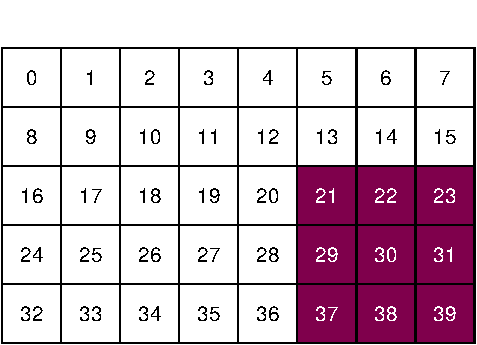
\includegraphics[width=0.8\textwidth]{arraygraphics_2_wo}}%
  \only<2>{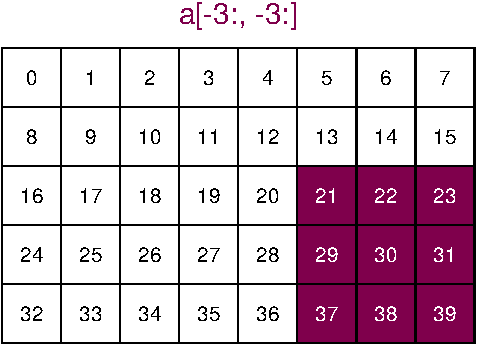
\includegraphics[width=0.8\textwidth]{arraygraphics_2}}%
  \only<3>{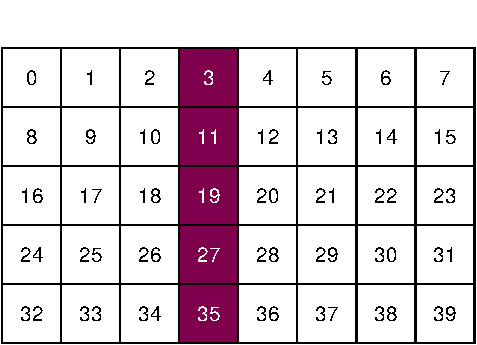
\includegraphics[width=0.8\textwidth]{arraygraphics_3_wo}}%
  \only<4>{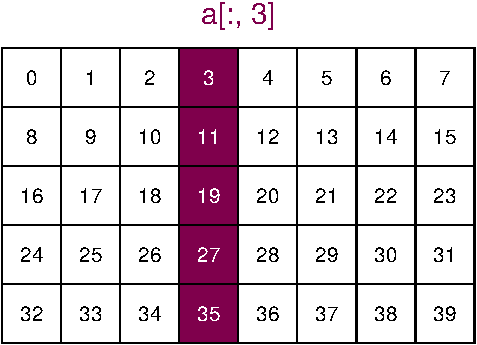
\includegraphics[width=0.8\textwidth]{arraygraphics_3}}%
  \only<5>{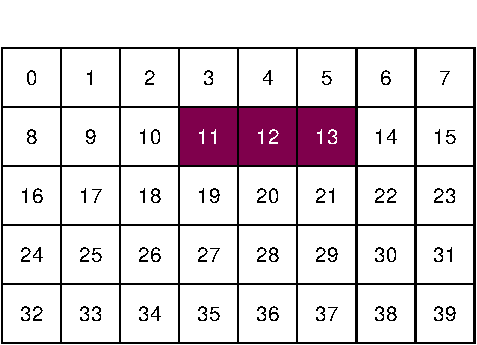
\includegraphics[width=0.8\textwidth]{arraygraphics_4_wo}}%
  \only<6>{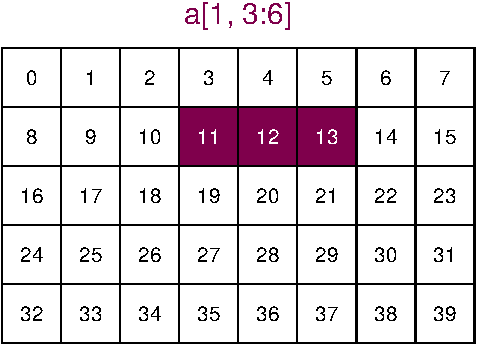
\includegraphics[width=0.8\textwidth]{arraygraphics_4}}%
  \only<7>{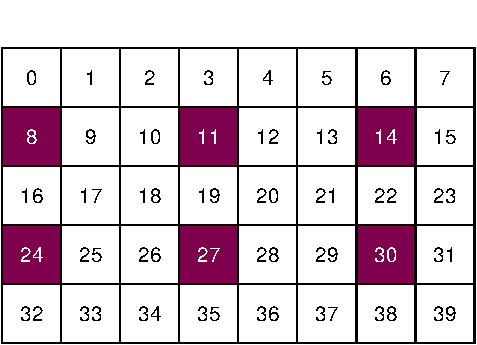
\includegraphics[width=0.8\textwidth]{arraygraphics_5_wo}}%
  \only<8>{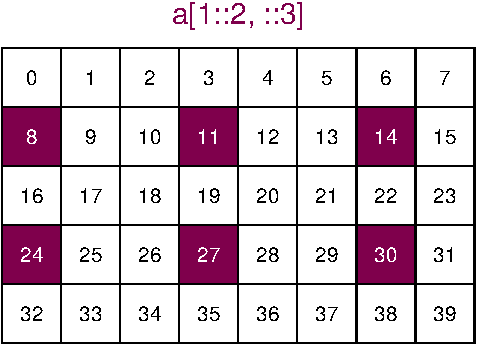
\includegraphics[width=0.8\textwidth]{arraygraphics_5}}
 \end{center}
\end{frame}

\begin{frame}{Fancy indexing -- Boolean mask}
 \begin{center}
  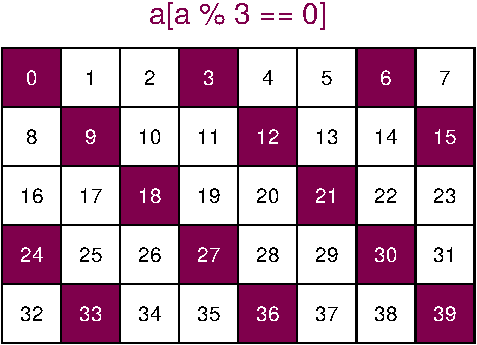
\includegraphics[width=0.8\textwidth]{arraygraphics_6}
 \end{center}
\end{frame}

\begin{frame}{Fancy indexing -- array of integers}
 \begin{center}
  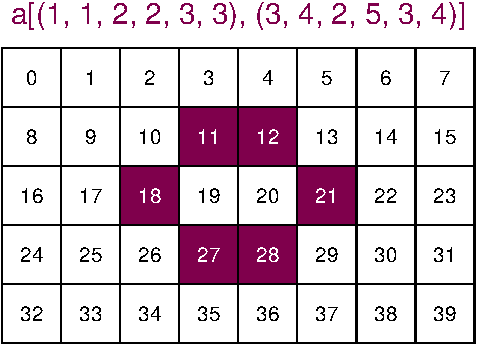
\includegraphics[width=0.8\textwidth]{arraygraphics_7}
 \end{center}
\end{frame}

\end{document}
